\documentclass[tikz,border=2pt]{standalone}
\usepackage{amsmath,amssymb}
\usepackage{pgfplots}
\pgfplotsset{compat=1.18}
\begin{document}
% Graphs of floor (blue, solid, closed left ends) and ceiling (red, dashed, closed right ends) on
% [-3,3], squeezed around y = x; at x = 2.7 the floor is 2 and the ceiling is 3.
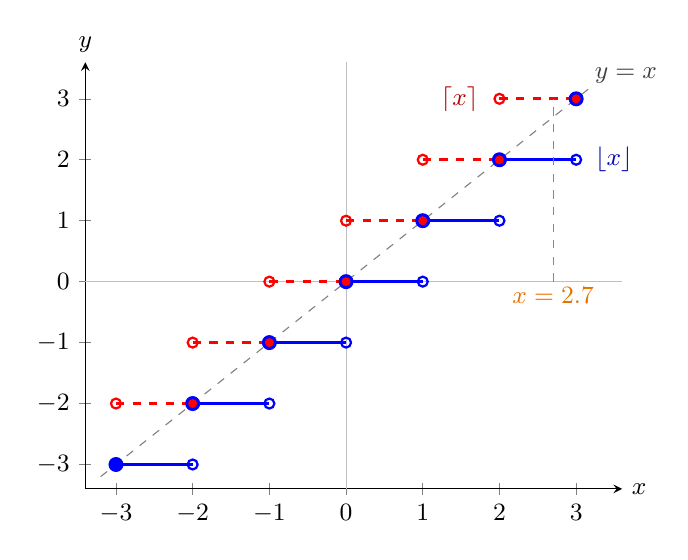
\begin{tikzpicture}[font=\small]
  \begin{axis}[
    axis lines=left,
    xmin=-3.4, xmax=3.6, ymin=-3.4, ymax=3.6,
    xtick={-3,...,3}, ytick={-3,...,3},
    xlabel={$x$}, ylabel={$y$},
    xlabel style={at={(axis description cs:1,0)}, anchor=west},
    ylabel style={rotate=-90, at={(axis description cs:0,1)}, anchor=south},
    width=8.4cm, height=7cm, clip=false
    ]
    \draw[gray!50, thin] (axis cs:-3.4,0) -- (axis cs:3.6,0);
    \draw[gray!50, thin] (axis cs:0,-3.4) -- (axis cs:0,3.6);
    \addplot[gray, thin, dashed, domain=-3.2:3.2] {x};
    \node[gray!50!black, anchor=south west, inner sep=1pt] at (axis cs:3.2,3.2) {$y=x$};
    % floor: [n, n+1) at height n
    \foreach \n in {-3,...,2} {
      \edef\tmp{\noexpand\addplot[blue, very thick] coordinates {(\n,\n) (\n+1,\n)};}\tmp
      \edef\tmp{\noexpand\addplot[only marks, mark=o, mark size=1.8pt, blue, thick, fill=white] coordinates {(\n+1,\n)};}\tmp
    }
    % ceiling: (n-1, n] at height n
    \foreach \n in {-2,...,3} {
      \edef\tmp{\noexpand\addplot[red, very thick, dashed] coordinates {(\n-1,\n) (\n,\n)};}\tmp
      \edef\tmp{\noexpand\addplot[only marks, mark=o, mark size=1.8pt, red, thick, fill=white] coordinates {(\n-1,\n)};}\tmp
    }
    % closed ends: at each integer both graphs take the value n (blue ring around red dot)
    \foreach \n in {-3,...,3} {
      \edef\tmp{\noexpand\addplot[only marks, mark=*, mark size=2.5pt, blue] coordinates {(\n,\n)};}\tmp
    }
    \foreach \n in {-2,...,3} {
      \edef\tmp{\noexpand\addplot[only marks, mark=*, mark size=1.4pt, red] coordinates {(\n,\n)};}\tmp
    }
    \node[blue!70!black, anchor=west] at (axis cs:3.12,2.0) {$\lfloor x\rfloor$};
    \node[red!70!black, anchor=east] at (axis cs:1.85,3.0) {$\lceil x\rceil$};
    % the example x = 2.7
    \draw[orange!90!black, thin, dashed] (axis cs:2.7,0) -- (axis cs:2.7,3);
    \node[orange!90!black, anchor=north, inner sep=2pt] at (axis cs:2.7,0) {$x=2.7$};
  \end{axis}
\end{tikzpicture}
\end{document}
